%%%%%%%%%%%%%%%%%%%%%%%%%%%%%%%%%%%%%%%%%%%%%%%%%%%
%% P3: Phenomenology of Particle Physics                         
%%
%% Author:  André Rubbia                   		 
%%
%% Figure 5.3 Comparison of the energy in the center-of-mass system (CMS),  in collider and fixed target (FT) modes.
%%
%% This work is licensed under the Creative Commons Attribution 4.0 International License. 
%% To view a copy of this license, visit http://creativecommons.org/licenses/by/4.0/ or 
%% send a letter to Creative Commons, PO Box 1866, Mountain View, CA 94042, USA.
%%
%%%%%%%%%%%%%%%%%%%%%%%%%%%%%%%%%%%%%%%%%%%%%%%%%%%

\documentclass[a4paper,10pt]{article}

\usepackage[T1]{fontenc}
\usepackage[utf8]{inputenc}
\usepackage{lmodern}
\usepackage[labelfont=bf]{caption}
\usepackage{upgreek}

\usepackage{tikz}
\usepackage{pgfplots}
\pgfplotsset{compat=1.17}
\usepgfplotslibrary{ternary}
\usepgfplotslibrary{fillbetween}
\usepgfplotslibrary{external}

\def\d{\mathrm{d}}

\begin{document}

%%%%%%%%%%%%%%%%   FIGURE  %%%%%%%%%%%%%%%%%%%%%%%%%%%%%%
\begin{figure}[htb]
\begin{center}
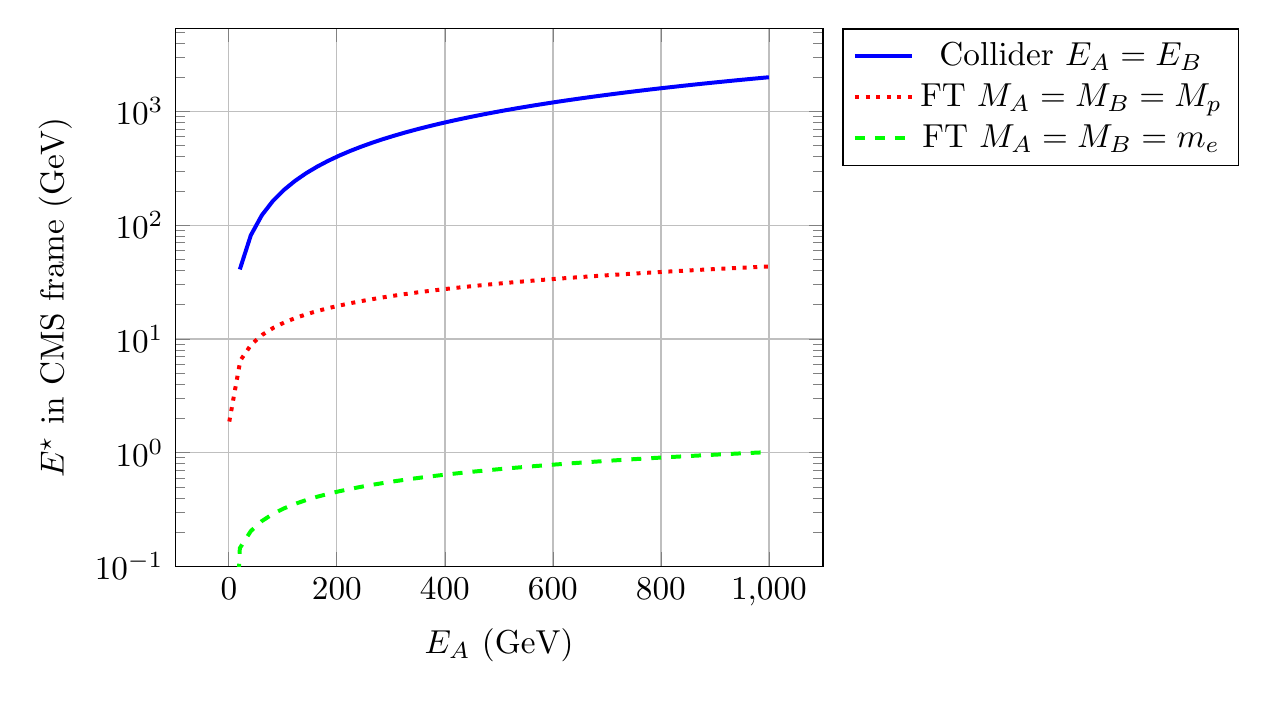
\begin{tikzpicture}[scale=1.2]
\begin{semilogyaxis}[
%xmin=0, xmax=180,
	grid=major,
%	ytick={0,45,90,135,180},
	ymin=1e-1,
	xlabel=$E_A$ (GeV),
	ylabel=$E^\star$ in CMS frame (GeV),
	legend entries={Collider $E_A=E_B$, FT $M_A=M_B=M_p$, FT $M_A=M_B=m_e$},
	legend pos = outer north east]
	\addplot[blue,domain=0:1000,very thick,samples=50,no marks] {2*x};
	\addplot[red,domain=0.938:1000,very thick,samples=50, no marks, dotted] {sqrt(2*0.938^2 + 2*0.938*x};
	\addplot[green,domain=0.511e-3:1000,very thick,samples=50,no marks, dashed] {sqrt(2*0.511e-3^2+2*0.511e-3*x};
\end{semilogyaxis}
\end{tikzpicture}
\caption{Comparison of the energy $E^\star$ in the center-of-mass system (CMS),  in collider and fixed target (FT) modes.
For the FT, the cases of electrons and protons are assumed.}
\end{center}
\end{figure}
%%%%%%%%%%%%%%%%   END FIGURE  %%%%%%%%%%%%%%%%%%%%%%%%%%%%%%
%

\end{document}
